\setcounter{equation}{0}
\chapter{Introduction}

\nomenclature{AI}{Artificial Intelligence}
\nomenclature{CUSAT}{Cochin University of Science and Technology}
\nomenclature{ML}{Machine Learning}
\nomenclature{IoT}{Internet of Things}
\nomenclature{CCTV}{Closed-Circuit Television}
\nomenclature{AOAV}{Action on Armed Violence}

\setlength{\parskip}{2ex}

\noindent In today's interconnected and increasingly complex world, safeguarding public safety has become critical to governments, law enforcement agencies, and communities globally. In the middle of many challenges faced by modern societies, the rise in violent incidents presents a particularly pressing threat, with outbreaks of unrest and disorder occurring all too frequently. Recognizing the urgency of addressing this issue, this work advocates for the integration of AI and deep learning technologies into public safety frameworks\cite{ai_saftey}. The percentage change in peace score from the year 2008 to 2023 is shown below in Figure \ref{fig:gpi1}.

\begin{figure}[htbp!]
    \centering
    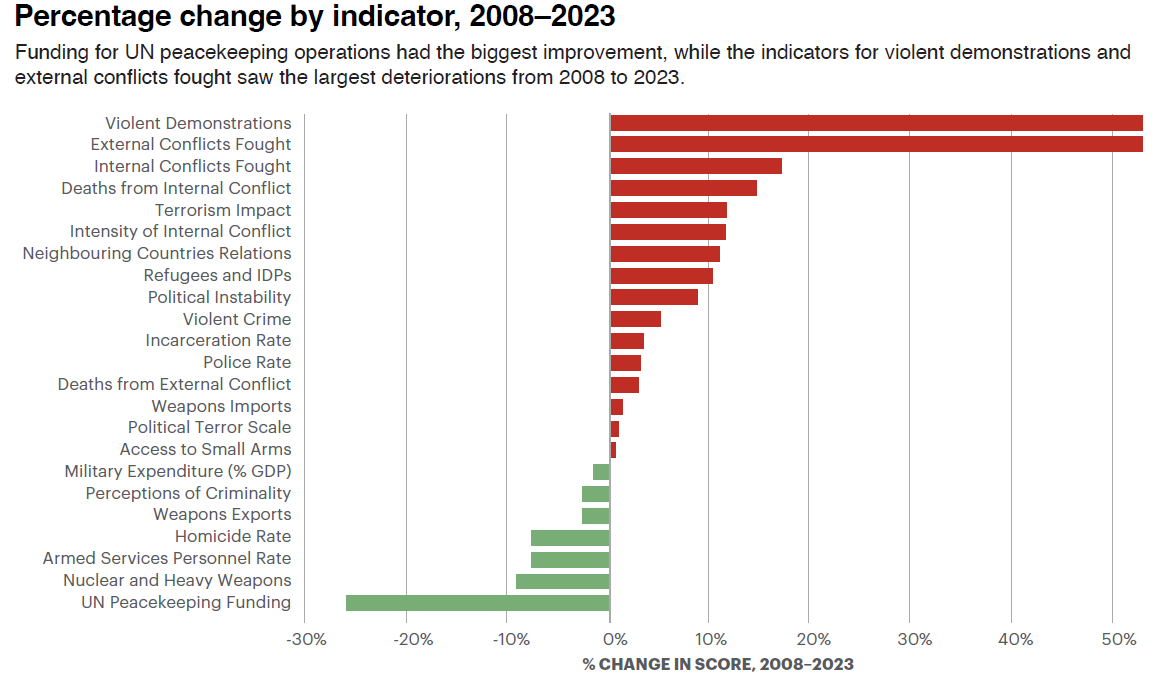
\includegraphics[width=0.875\linewidth]{Images/gpi 1.png}
    \caption{Percentage Change by Indicator, 2008–2023}
    %\renewcommand{\label}[1]{}
    \label{fig:gpi1}
\end{figure}

\noindent Figure \ref{fig:gpi1} shows that while there's been a positive development with a 50\% increase in funding for UN peacekeeping, a closer look reveals a concerning trend. Since 2008, the world has grown less peaceful. Indicators surrounding conflict paint an unapproachable picture: a rise in violent demonstrations, an increase in the number of external and internal conflicts fought, and a surge in deaths caused by external conflicts. Furthermore, the number of refugees and instances of political instability have grown significantly. However, there are a few flashes of hope. Relations between neighboring countries have shown slight improvement, and there have been small decreases in both police rates and prison rates. Overall, the data suggests a world in need of solutions to promote peace and stability.

\noindent By harnessing the analytical skills of AI algorithms and the predictive capabilities of deep learning models, the team proposes a transformative approach to the detection and prevention of violence. The methodology involves the aggregation and analysis of data from diverse sources, including surveillance systems, social media platforms, and sensor networks. Through sophisticated data processing and pattern recognition techniques, the framework aims to identify early warning signs of potential disturbances, enabling proactive intervention by law enforcement agencies and security personnel. The strategic deployment of AI-driven insights and intervention strategies holds the promise of empowering authorities to anticipate and defuse volatile situations before they escalate into violence. By leveraging advanced predictive analytics and situational awareness tools, the framework seeks to enhance the effectiveness and efficiency of public safety efforts, thereby minimizing the risk of harm to individuals and communities.

\noindent Moreover, this work underscores the importance of considering ethical considerations and societal implications in the adoption of AI for violence detection and prevention\cite{crowd_viol}. As with any technology, the responsible use of AI requires careful attention to issues such as privacy, bias, and accountability. By addressing these concerns and encouraging transparency and accountability in AI-driven decision-making processes, therefore it ensures that efforts to enhance public safety are aligned with fundamental principles of justice and human rights.

\clearpage

\noindent The integration of cutting-edge technologies, particularly AI, holds the key to reshaping public safety and security. Embracing these advancements and promoting collaboration among diverse stakeholders, including government bodies, law enforcement agencies, technologists, and communities, is essential. By prioritizing inclusivity and equity in AI development it ensures the needs of all members of society, paving the way for safer, more resilient communities characterized by trust, transparency, and vibrant social interaction.


\setlength{\parskip}{2ex}

\section{Background and Motivation}

% \section{Background}

\noindent Violence, in its various forms, presents significant threats to public safety, organizational security, and individual well-being. Incidents of violence occur in diverse settings, including public spaces, workplaces, and homes, resulting in severe consequences such as injuries, fatalities, and infrastructure damage. Violence not only harms its direct victims but also spreads a broad impact on society. The trend in the global economic impact of violence through the years 2008 to 2022 is shown below in Figure \ref{fig:gpi2}

\begin{figure}[htbp!]
    \centering
    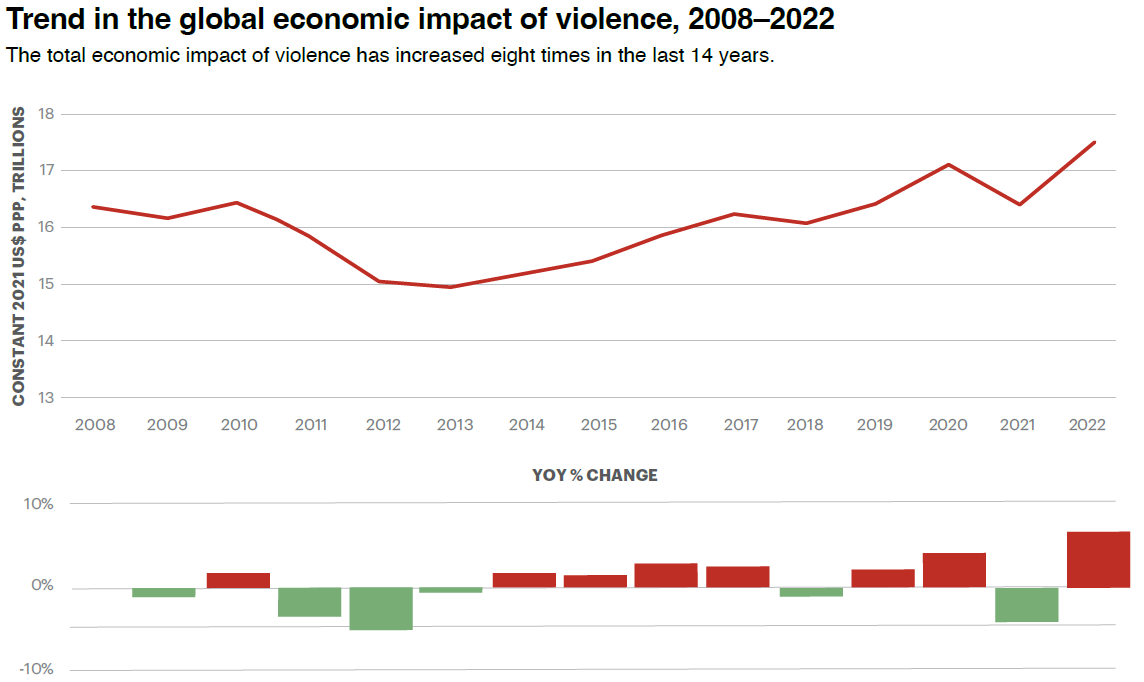
\includegraphics[width=1\linewidth]{Images/gpi 2.png}
    \caption{Trend in the Global Economic Impact of Violence, 2008–2022}
    %\renewcommand{\label}[1]{}
    \label{fig:gpi2}
\end{figure}

\noindent On analyzing Figure \ref{fig:gpi2}, in 2008 the economic impact of violence was estimated to be around \$10 trillion (in constant 2021 US dollars). By 2022, the economic impact of violence had increased to around \$18 trillion. This represents an increase of 80\% over the period. The graph also shows the economic impact of violence has increased significantly, such as in 2017(10\%) and the economic impact of violence has decreased, in 2012(by 10\%).

\noindent The primary effect of violence is that it breaks down trust and unity among communities. When individuals feel unsafe in their neighborhoods or workplaces, social interactions become strained, and community bonds weaken. Fear of violence can lead to social isolation and increase feelings of loneliness.

\noindent Additionally, violent incidents impose substantial economic burdens on society, involving costs associated with medical treatment, criminal justice proceedings, and victim rehabilitation services. Violent activities are not only between humans, humans to animals, and animals to humans, but human to materials is also possible. For example, if a stressed person breaks down a pipeline in a factory can cause injuries to others as well. Hence, it brings the need to prevent violent incidents as soon as possible before they go to extreme conditions.

\noindent Violent incidents among the public can be identified through surveillance cameras\cite{violence_ai}. Despite advancements in video analysis, many surveillance systems still rely on human operators to monitor live feeds or review recorded footage. This process can be labor-intensive and prone to errors, as operators may miss violent incidents due to factors like fatigue, distractions, or the sheer volume of footage to review.

\noindent Even if a violent incident is captured on camera, the effectiveness of the response depends on how quickly it's detected and acted upon. Manual monitoring may not always ensure timely intervention, allowing incidents to escalate before appropriate measures are taken\cite{manual_Violence}. As a result, it is very essential to develop a system that can leverage cutting-edge technologies to enhance the detection and timely alerting for the prevention of violence. This can be achieved through leveraging the power of AI, machine learning, and computer vision techniques which enable the system to analyze live video feeds or recorded footage to automatically identify violent behaviors or patterns associated with the video.

\clearpage

\section*{Motivation}

\noindent The motivation behind the development of a violence detection system is followed by real-life incidents that highlight the urgent need for improved methods for early analyzing and alerting the possible violent incidents that can happen in public spaces, which helps the relevant authorities take action to prevent them. One such incident that exemplifies this need is the tragic stampede that occurred during a cultural festival at Cochin University of Science and Technology (CUSAT) on 25th November 2023. A news clip of the same incident is shown in Figure \ref{CUSAT}\\

\begin{figure}[htbp!]
    \centering
    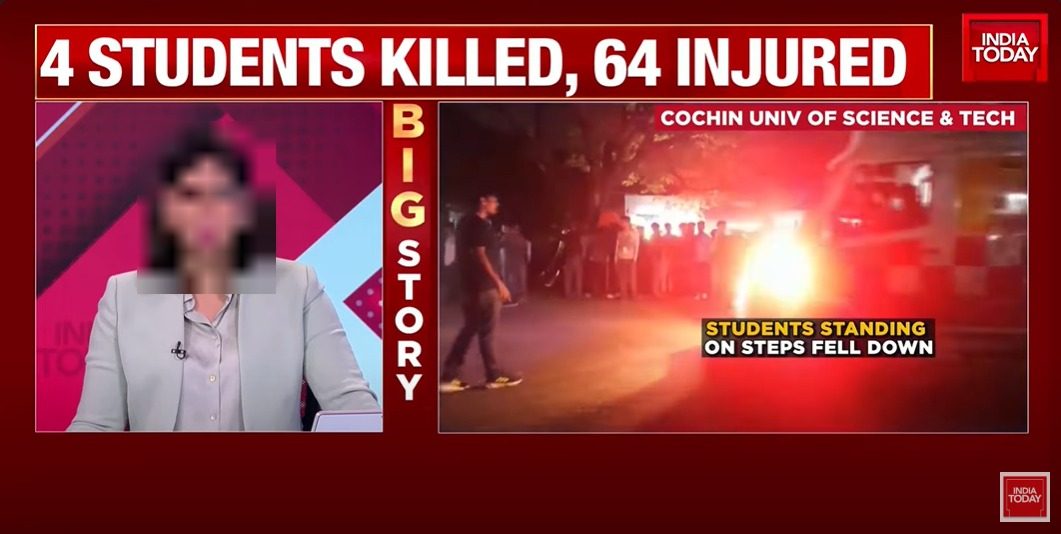
\includegraphics[width=1\linewidth]{Images/stampede.png}
    \caption[NEWS Clip of the CUSAT Stampede Incident]{NEWS Clip of the CUSAT Stampede Incident, November 25, 2023, by India Today NEWS Channel}
    \label{CUSAT}
\end{figure}

\noindent The CUSAT stampede, which resulted in multiple fatalities and injuries, was a reminder of the potential consequences of overcrowding, mismanagement, and the rapid escalation of violence in crowded environments. What began as a festive celebration quickly overturn into chaos and panic, as attendees struggled to navigate overcrowded pathways and exits, leading to a stampede that claimed the lives of innocent individuals.

\clearpage

\noindent This tragic event not only reminds the limitations of existing security measures but also highlights the need for more advanced technologies AI, ML, etc in detecting and mitigating violence in real time. Traditional methods were mostly reactive, meaning they would respond after something bad had already happened\cite{manual_Violence}. This delay made it harder to prevent violence from getting worse. Also, modern cities are so complex, with lots of people and different cultures mixing, which makes it even tougher for authorities to keep an eye on things. That's where AI steps in. It's like having a super-smart detective that can analyze tons of different data in real-time, like security camera footage and sensor readings\cite{ai_saftey}. When AI detects unusual behavior or signs of trouble early, it can alert the relevant authorities, enabling them to step in and prevent the situation from escalating.

\noindent Action on Armed Violence (AOAV) records, investigates, and disseminates evidence of armed violence against civilians worldwide, to ensure the respect and protection of their rights and to end armed violence against civilians in conflict. Some of the records of information are mentioned below in Table \ref{ann_casualties} and Table \ref{AOAV} and Figure \ref{AOAVfig}: 

\begin{table}[htbp!]
  \centering
  \caption{Annual Casualties Caused by Violence}
  \begin{tabular}{l|c}
    \hline
    Year & Total \\
    \hline
    2022 & 6,886 \\
        % \hline
    2023 & 15,305 \\
        \hline
    \end{tabular}
    \label{ann_casualties}
\end{table}


\begin{table}[htbp!]
  \centering
  \caption{Key Findings and Percentage of Violence Table}
  \begin{tabular}{|p{12cm}|p{3cm}|}
    \hline
    \textbf{Key Findings} &  \textbf{Percentage} \\
    \hline
    Air-launched attacks & 226\% \\
    \hline
    Increase in civilian fatalities vs. 2022 & 122\% \\
    \hline
    \% of civilians harmed in towns/cities & 90\% \\
    \hline
    \% of civilians harmed in populated areas & 90\% \\
    \hline
    \% of civilian casualties from state actors & 77\% \\
    \hline
    \% of violence incidents in populated areas & 76\% \\
    \hline
    Rise in explosive weapon use & 69\% \\
    \hline
    \% of civilian fatalities from air strikes & 67\% \\
    \hline
    Ground-launched attacks & 56\% \\
    \hline
  \end{tabular}
  \label{AOAV}
\end{table}

\begin{figure}[!htbp]
    \centering
    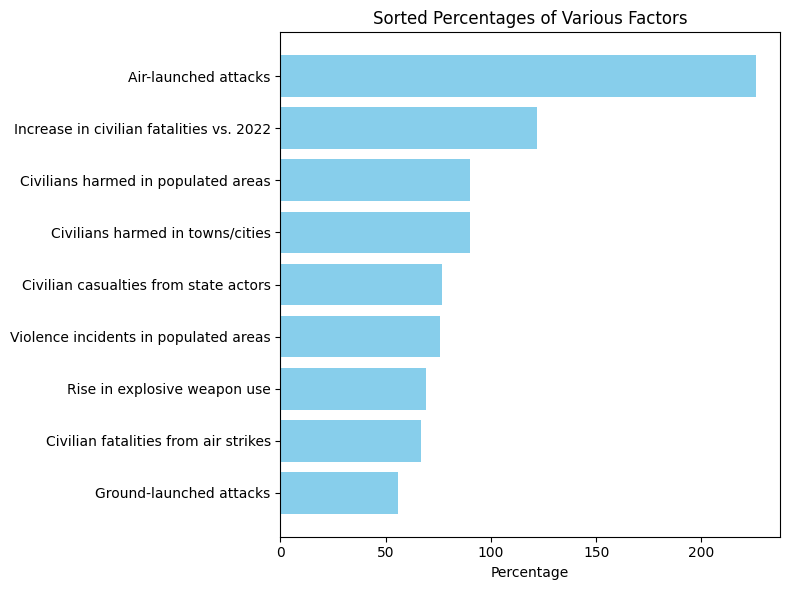
\includegraphics[width=1\linewidth]{Images/violent_behaviors.png}
    \caption[Key Findings and Percentage of Violence Graph]{Graphical Representation of the Above Table}
    %\renewcommand{\label}[1]{}
    \label{AOAVfig}
\end{figure}

\noindent The key findings from the global explosive violence monitor report by Action on Armed Violence underscore a concerning escalation in civilian casualties and incidents of explosive weapon use worldwide in 2023. The significant increase in civilian fatalities, a rise in explosive weapon use, and the prevalence of air-launched attacks highlight the devastating impact of modern warfare tactics on civilian populations, particularly in populated areas. The report also emphasizes the disproportionate harm suffered by civilians, with the majority of those harmed being non-combatants, and the alarming trend of state actors being responsible for a significant portion of civilian casualties. These findings underscore the urgent need for concerted efforts to mitigate the impact of explosive violence and protect civilian lives in conflict-affected regions worldwide.

\clearpage

\section{Objective and Scope}

% \section{Objective}

The development of robust and efficient models for violence detection from video is crucial for ensuring public safety and security. However, existing models often face challenges such as overfitting, complexity, and resource-intensive requirements, limiting their deployment in systems with limited specifications\cite{overfit}. So the objectives of the project are:

\begin{itemize}
    \item \textbf{Addressing Overfitting:} Overfitting is a common issue in existing systems and occurs when a machine learning model learns the training data too well but performs poorly on unseen data. So the aim is to develop a model that is less prone to overfitting, thereby improving its generalization capability\cite{overfit}.

    \item \textbf{Designing a Less Complex system:} The intention is to create a neural network that is less complex when compared to existing architectures. Beginning with a CNN-LSTM model, the aim is to refine it into an enhanced version that aligns with the objectives.

    \item \textbf{Enhancing Model Accessibility:} Due to the reasonably compact architecture of the proposed network, it can be trained and deployed on systems with reasonable specifications, thus increasing accessibility and cost-effectiveness.

    \item \textbf{Comparison with Highly Sophisticated Models:} Unlike highly sophisticated models that necessitate high-end systems for training and processing, the proposed network provides a more feasible alternative. Highly sophisticated models often demand extensive computational resources and may not be feasible for deployment on standard hardware. By prioritizing simplicity and efficiency, the proposed approach aims to reduce the gap between cutting-edge research and practical implementation.

    \item \textbf{Suitability for Edge Devices:} The model's reduced size and complexity make it well-suited for implementation on edge devices, including surveillance cameras, Internet of Things (IoT) devices, and more\cite{edge_ai}. This enables efficient deployment in real-world scenarios, enhancing its practical utility.
\end{itemize}

\clearpage

\section*{Scope}


\noindent The project aims to develop a robust system for violence detection and classification of corresponding actions as violent or not, utilizing machine learning and computer vision techniques to analyze videos. Its primary objective is to identify instances of physical confrontations or riots involving two or more parties. Upon detection, the system can be modified to notify relevant authorities promptly, facilitating timely intervention and resolution of disputes. By automating the process of detecting and categorizing violent incidents, the system seeks to contribute to the maintenance of law and order, ultimately enhancing safety and security in public spaces\cite{in_out_violence_ai}.

\noindent In line with enhancing safety and security, the project seeks to create a tool for monitoring and responding to potential threats. By deploying an intelligent surveillance system equipped with violence detection algorithms, the project aims to enable law enforcement agencies to stay ahead of security threats, thereby reducing the likelihood of violence and enhancing overall public safety. 

\noindent The project's motivations are grounded in the prevention of criminal activities through timely intervention and the protection of vulnerable spaces. By intervening at the earliest stage, the project aims to disrupt criminal activities before they escalate, contributing to the reduction of crime rates such as assaults, vandalism, and riots. Moreover, by enhancing surveillance capabilities in high-risk areas, authorities can effectively monitor sensitive locations, reducing vulnerability to criminal activities and ensuring safety. Ultimately, the project seeks to promote community well-being by fostering trust, cohesion, and social harmony through the creation of safer and more secure environments. Through the empowerment of law enforcement agencies, the project aims to strengthen their capacity to protect and serve the community, enhancing public confidence to maintain safety and security.

\clearpage

\section{Contributions}
% \vspace{-10mm}
% \small Rewritten

\noindent The project makes significant strides in the domain of public safety and violence prevention through a series of key initiatives. Primarily, the development of an advanced AI model tailored explicitly for detecting violence in video content\cite{comp_vision}. This model incorporates techniques in deep learning and computer vision, ensuring precise analysis of video data to identify potential instances of violence. By leveraging AI algorithms, the proposed system offers an approach to threat identification and violence prevention, which is crucial for maintaining public safety.

\noindent Additionally, the project emphasizes the integration of data analysis capabilities, facilitating continuous monitoring of various data sources including surveillance cameras, social media platforms, and sensor networks\cite{Data_integrat}. This empowers law enforcement and security personnel to detect early signs of potential disturbances, enabling timely intervention to uphold public safety and order. 

\noindent Together with technological advancements, ethical considerations, and accountability remain central to the project aim, prioritizing the development and deployment of the AI-powered violence detection system in accordance with ethical principles and individual rights\cite{ai_ethics}. The framework incorporates robust safeguards to mitigate risks such as privacy breaches and algorithmic biases, ensuring responsible and ethical operation.

\noindent Moreover, the project offers scalability and adaptability for flexible solutions adaptable to diverse contexts and environments. The modular design of the framework facilitates integration with existing public safety infrastructure and allows for customization to meet specific needs. This scalability and adaptability guarantee safer and more resilient communities.

\noindent The project endeavors to contribute to public safety and community welfare by leveraging AI technologies for detecting and preventing violence. It aims to offer authorities actionable insights and intervention strategies, envisioning safer public spaces conducive to peaceful coexistence\cite{public_sector_ai}. The project seeks to cultivate safer communities and foster harmony in society, aspiring to create a more secure environment for future generations.

\lfoot{\textit{Departmant of Artificial Intelligence and Data Science, SJCET Palai}}
\renewcommand{\footrulewidth}{0.4pt}